% Centri — end-to-end walkthrough (for the advisor: educational-technology / stats focus)
% Compile: pdflatex -interaction=nonstopmode centri-end-to-end.tex   (run twice)
\documentclass[aspectratio=169,10pt]{beamer}
\usetheme{metropolis}
\metroset{sectionpage=progressbar, subsectionpage=none, numbering=fraction, progressbar=frametitle}

\usepackage{booktabs}
\usepackage{amsmath,amssymb}
\usepackage{siunitx}
\usepackage{xcolor}
\usepackage{graphicx}
\graphicspath{{figs/}}
\usepackage{tikz}
\usetikzlibrary{arrows.meta,positioning,calc,shapes.geometric,fit,backgrounds}
\usepackage[most]{tcolorbox}

% ---- palette -------------------------------------------------------------
\definecolor{cMeas}{HTML}{1F6FB2}
\definecolor{cPed}{HTML}{B5651D}
\definecolor{cApp}{HTML}{2E7D32}
\definecolor{cInfra}{HTML}{5E35B1}
\definecolor{cAccent}{HTML}{C62828}
\definecolor{cGrey}{HTML}{616161}
\definecolor{cBg}{HTML}{F4F6F8}
\setbeamercolor{frametitle}{bg=cMeas}
\setbeamercolor{progress bar}{fg=cAccent}

% ---- a "big number" callout ---------------------------------------------
\setlength{\fboxrule}{0.8pt}
\newcommand{\bignum}[2]{%
  \fcolorbox{cMeas}{cMeas!10}{\parbox[t]{25mm}{\centering
    {\bfseries\large\color{cMeas} #1}\\[1pt]{\scriptsize #2}\strut}}}
\newcommand{\hl}[1]{{\bfseries\color{cAccent}#1}}

% ---- tikz styles ---------------------------------------------------------
\tikzset{
  box/.style={rounded corners=2pt, draw=#1, line width=0.8pt, fill=#1!8,
              text=black, align=center, font=\scriptsize, inner sep=4pt, minimum height=7mm},
  node distance=6mm and 9mm,
  flow/.style={-{Stealth[length=2.2mm]}, line width=0.7pt, draw=cGrey},
  hot/.style={-{Stealth[length=2.6mm]}, line width=1.0pt, draw=cAccent},
  lbl/.style={font=\tiny\itshape, text=cGrey, fill=white, inner sep=1pt},
}

\title{Centri: from one video to physics and personalised pedagogy}
\subtitle{System walkthrough --- methods, measurements, evaluation}
\author{Damar Albaribin}
\institute{MSc Thesis --- advisor: Prof.\ Wu-Yuin Hwang}
\date{\today}

\begin{document}
\maketitle

\begin{frame}{From each case to grounded learning material (real, generated)}
\scriptsize Each scene's measured numbers ground the explanation; the narration follows the actual motion regime.
\vspace{0.4em}
\begin{columns}[T]
\column{0.33\textwidth}
\textbf{\color{cApp}Bicycle} --- uniform\\{\tiny ``what the video shows over time''}
\vspace{2pt}\par
\emph{``The wheel turns at a steady rate; $\omega$ stays near \hl{5.1\,rad/s}, so the period holds at \hl{1.18\,s} --- uniform circular motion.''}
\column{0.33\textwidth}
\textbf{\color{cAccent}Turntable} --- decelerating\\{\tiny ``how the variables relate''}
\vspace{2pt}\par
\emph{``After the push the disk coasts down; $\omega$ falls, and since $a_c=\omega^2 r$, the inward acceleration drops with it.''}
\column{0.33\textwidth}
\textbf{\color{cPed}Fan} --- accelerating\\{\tiny ``what the video shows over time''}
\vspace{2pt}\par
\emph{``At $t\!\approx\!1$\,s, $\omega$ is \hl{1.99\,rad/s}; by $t\!\approx\!7$\,s it is \hl{9.77} --- a steady spin-up, $\alpha=$\hl{1.18\,rad/s$^2$}.''}
\end{columns}
\vspace{0.5em}
{\scriptsize The non-uniform cases let the material teach angular acceleration \emph{from the phenomenon} --- something a steady spin (or a generic textbook) cannot.}
\end{frame}

% =========================================================================
\section{Method 2 --- Generation (physics $\rightarrow$ pedagogy)}

\begin{frame}{Grounded, multimodal learning-material generation}
\begin{columns}[T]
\column{0.55\textwidth}
\small
Each measured scene yields one \hl{authentic learning passage}, written by the language model
but grounded strictly in the scene's real numbers, in \hl{five} sections:
\begin{itemize}\setlength\itemsep{1pt}
  \item \textbf{Scenario} --- a short, \hl{student-centred story} that opens with \emph{why it
  matters}, answers \emph{who\,/\,what\,/\,when\,/\,where\,/\,why\,/\,how} (5W$+$1H), and names an
  \emph{authentic daily-life context} (e.g.\ ``Irfan rode his bike across town'') --- not just object\,/\,axis\,/\,clip length
  \item \textbf{Variables} --- $r,\omega,v,a_c,T,f$ (and $\alpha$) defined + measured
  \item \textbf{Relationships} --- $v=\omega r$, $a_c=\omega^2 r$, checked on the numbers \emph{and shown through annotation} (image\,/\,graph\,/\,table), not prose alone
  \item \textbf{Over time} --- narrates $\omega(t)$ from the actual clip
  \item \textbf{Figures} --- reads the annotated image / graph / table
\end{itemize}
A \textbf{deterministic seed} hands the model the variables, formula relations and a
time-anchored $\omega(t)$, so the prose is fluent but \alert{never invents a number}.
\column{0.45\textwidth}
\centering
{\footnotesize \textbf{Seed (truth) $\to$ model (prose):}}\\[4pt]
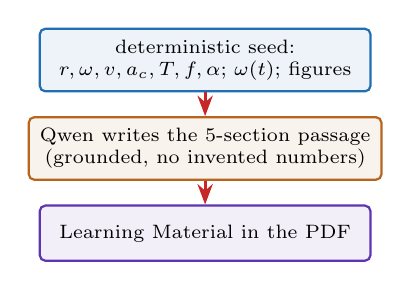
\begin{tikzpicture}[node distance=3mm]
  \node[box=cMeas, minimum width=42mm] (s) {\scriptsize deterministic seed:\\$r,\omega,v,a_c,T,f,\alpha$; $\omega(t)$; figures};
  \node[box=cPed, below=of s, minimum width=42mm] (m) {\scriptsize Qwen writes the 5-section passage\\(grounded, no invented numbers)};
  \node[box=cInfra, below=of m, minimum width=42mm] (p) {\scriptsize Learning Material in the PDF};
  \draw[hot] (s)--(m); \draw[hot] (m)--(p);
\end{tikzpicture}\\[4pt]
{\scriptsize Multimodal: the passage refers to the same \texttt{image\,/\,graph\,/\,table} the figures provide.}
\end{columns}
\vspace{-0.2em}
{\scriptsize The material teaches the concept \emph{from this specific phenomenon} --- the grounding a generic textbook cannot supply, and exactly what the evaluation measures.}
\end{frame}

\begin{frame}{One scene, four modalities --- the actual stimuli}
\centering
\begin{columns}[T]
\column{0.33\textwidth}\centering
\begin{minipage}[c][0.46\textheight][c]{\linewidth}\centering
  \includegraphics[width=\linewidth,height=0.46\textheight,keepaspectratio]{fan_annotated_image}\end{minipage}\\[3pt]
{\scriptsize \textbf{\color{cMeas}image} --- read geometry off the annotated frame}
\column{0.33\textwidth}\centering
\begin{minipage}[c][0.46\textheight][c]{\linewidth}\centering
  \includegraphics[width=\linewidth,height=0.46\textheight,keepaspectratio]{fan_annotated_graph}\end{minipage}\\[3pt]
{\scriptsize \textbf{\color{cMeas}graph} --- read $\omega(t)$ values / trend}
\column{0.33\textwidth}\centering
\begin{minipage}[c][0.46\textheight][c]{\linewidth}\centering
  \includegraphics[width=\linewidth,height=0.46\textheight,keepaspectratio]{fan_annotated_table}\end{minipage}\\[3pt]
{\scriptsize \textbf{\color{cMeas}table} --- look up a measured quantity}
\end{columns}
\vspace{0.4em}
{\scriptsize A fourth \textbf{\color{cMeas}text} modality states the numbers inline. The learning material refers to each of these, so a text-only vs.\ text$+$visual presentation is built in. All three panels are real pipeline figures for the same fan scene.}
\end{frame}

\begin{frame}{The pedagogy seam: worksheet and interactive tutor}
\centering
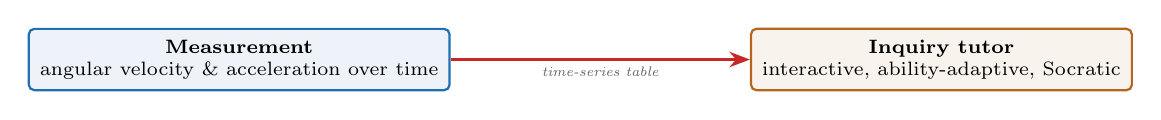
\begin{tikzpicture}[node distance=6mm and 16mm]
  \node[box=cMeas, minimum width=34mm] (m) {\textbf{Measurement}\\angular velocity \& acceleration over time};
  \node[box=cPed, right=38mm of m, minimum width=36mm] (p) {\textbf{Inquiry tutor}\\interactive, ability-adaptive, Socratic};
  \draw[hot] (m)--(p) node[lbl,midway,below=1pt]{time-series table};
\end{tikzpicture}
\vspace{0.6em}
\begin{exampleblock}{\small From two captures to one}
{\small A sensor-based protocol needs \alert{two} acts --- an \emph{image} (object, centre, radius)
\emph{and} a \emph{gyroscope} recording. One video supplies \alert{both at once}:
it does not merely substitute the sensor, it \emph{collapses the two captures into one} --- a simpler protocol for the learner.}
\end{exampleblock}
\vspace{0.3em}
{\footnotesize \textbf{Material vs.\ tutor (a deliberate pedagogical distinction):}
the generated learning material is one-shot and identical every run; the inquiry tutor is interactive,
staged, adapts to a learner's ability band, and tracks misconceptions. The material \emph{complements} the tutor.}
\end{frame}

% =========================================================================
\section{Method 3 --- Evaluation (the statistics)}

\begin{frame}{Evaluation methodology --- what we measure and how}
\small
\begin{columns}[T]
\column{0.5\textwidth}
\textbf{\color{cMeas}Run now --- automatic relevance}
\begin{itemize}\setlength\itemsep{1pt}
  \item \textbf{Reference:} a real textbook section (OpenStax College Physics \S6.2), reorganized into our format --- independent of our pipeline \emph{(robustness now also checked against an independent set of \hl{19} English references)}
  \item \textbf{BERTScore} (P,\,R,\,F1): token-level cosine similarity in contextual embeddings --- kept \emph{for comparability with the prior method}
\end{itemize}
\column{0.5\textwidth}
\textbf{\color{cAccent}Planned --- quality (not yet run)}
\begin{itemize}\setlength\itemsep{1pt}
  \item \textbf{LLM-as-judge}: rubric scoring of correctness \& pedagogical quality (similarity $\ne$ quality)
  \item \hl{10}-teacher panel: clarity, correctness, level fit, usefulness --- mirrors the prior method
  \item reliability \textbf{Cohen's / Fleiss' $\kappa$}; comparison \textbf{ANOVA} (difficulty $\times$ modality); auto-vs-human \textbf{Pearson $r$}
\end{itemize}
\end{columns}
\vspace{0.4em}
{\scriptsize \textbf{Honest status:} so far we report \emph{relevance only} (BERTScore). The quality half --- the teacher panel and the LLM-judge --- is \emph{designed but not yet run}. That is by intent: BERTScore measures \emph{similarity}, not quality, so those sit on top of it. (Headline relevance number + breakdown: next slides.)}
\end{frame}

\begin{frame}{How the automatic score is computed}
\small
\begin{columns}[T]
\column{0.57\textwidth}
\textbf{BERTScore} --- relevance of the material to the reference
\begin{enumerate}\setlength\itemsep{2pt}\footnotesize
  \item embed every \emph{token} of candidate material $c$ and reference $r$ with a contextual model (RoBERTa-large) --- so ``wheel'' and ``tyre'' score as close
  \item greedily match each token to its best cosine counterpart:
\end{enumerate}
\vspace{-0.4em}
{\footnotesize\[
P=\tfrac{1}{|c|}\!\sum_{t\in c}\max_{s\in r}\cos(t,s),\;\;
R=\tfrac{1}{|r|}\!\sum_{s\in r}\max_{t\in c}\cos(s,t),\;\;
F_1=\tfrac{2PR}{P+R}
\]}
\vspace{-0.2em}
\begin{itemize}\setlength\itemsep{1pt}\footnotesize
  \item score the whole passage, and per section, against the same reference
\end{itemize}
\textbf{Per section} --- where the overlap is\\(diagnostic)
\begin{itemize}\setlength\itemsep{1pt}\footnotesize
  \item highest on \emph{``how the variables relate''} (\hl{0.855}) --- the formulas the textbook shares
  \item lower on the grounded sections --- our value-add the textbook lacks
\end{itemize}
\column{0.43\textwidth}
\centering
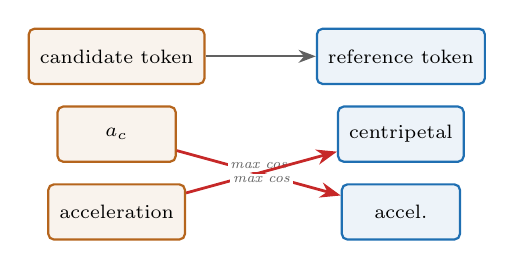
\begin{tikzpicture}[font=\tiny, node distance=2.6mm]
  \node[box=cPed, minimum width=15mm] (c1) {candidate token};
  \node[box=cPed, below=of c1, minimum width=15mm] (c2) {$a_c$};
  \node[box=cPed, below=of c2, minimum width=15mm] (c3) {acceleration};
  \node[box=cMeas, right=14mm of c1, minimum width=15mm] (r1) {reference token};
  \node[box=cMeas, below=of r1, minimum width=15mm] (r2) {centripetal};
  \node[box=cMeas, below=of r2, minimum width=15mm] (r3) {accel.};
  \draw[hot] (c2)--(r3) node[lbl,midway,above]{max cos};
  \draw[hot] (c3)--(r2) node[lbl,midway,below]{max cos};
  \draw[flow] (c1)--(r1);
\end{tikzpicture}
\vspace{4pt}
{\scriptsize \textbf{Current set} (5 runs / 3 phenomena: turntable\,$\times$3, bike, fan): whole-passage BERTScore \hl{F1\,0.840\,$\pm$\,0.002} vs.\ OpenStax \S6.2.}\\[3pt]
{\scriptsize The reference is real OpenStax \S6.2 --- \emph{reorganised} into our five sections (not the raw PDF, not paraphrased), built independently of our generation. \S6.2 is \emph{uniform} motion only, so we also score against an independent \hl{19}-source English reference set (universities / OER / worksheets) --- see the robustness band on the results slide.}
\end{columns}
\end{frame}

\begin{frame}{What is compared: our material vs.\ the reference (fan)}
\scriptsize
\textbf{Left} = our pipeline's generated learning material (Subagent D, grounded on the tracked fan clip). \textbf{Right} = the gold reference, OpenStax \S6.2, reorganised into the same five sections. BERTScore compares the two, section by section.
\vspace{0.4em}
\begin{columns}[T]
\column{0.5\textwidth}
\begin{tcolorbox}[colback=cPed!6,colframe=cPed!55,boxrule=0.4pt,left=3pt,right=3pt,top=2pt,bottom=2pt]
{\scriptsize\textbf{\color{cPed}Generated (ours) --- grounded in this fan}}
\end{tcolorbox}
\vspace{2pt}
{\tiny\textbf{Scenario.} A small yellow toy on a rotating fan blade traces a circular path, completing $\approx$\hl{7.7} revolutions over a 7\,s clip, counter-clockwise. \emph{Every number below comes from tracking the toy frame by frame at 60\,fps.}\par\vspace{3pt}
\textbf{How the variables relate.} $v=\omega r$; $a_c=\omega^2 r=v^2/r$, so doubling $\omega$ quadruples $a_c$; $T=1/f=2\pi/\omega$. Tangential $a_t=\alpha r=$\hl{0.53\,m/s$^2$}. \emph{The yellow toy supplies the measured values} ($r=$\hl{0.44\,m}, $\omega=$\hl{6.59}, $a_c=$\hl{21.8}).}
\column{0.5\textwidth}
\begin{tcolorbox}[colback=cMeas!6,colframe=cMeas!55,boxrule=0.4pt,left=3pt,right=3pt,top=2pt,bottom=2pt]
{\scriptsize\textbf{\color{cMeas}Reference (gold) --- OpenStax \S6.2}}
\end{tcolorbox}
\vspace{2pt}
{\tiny\textbf{Scenario.} An object moves in a circular path at constant speed --- uniform circular motion. Its direction changes constantly, so there is always an associated acceleration --- like feeling a sideways push when you turn a corner in a car.\par\vspace{3pt}
\textbf{How the variables relate.} For radius $r$ at speed $v$, $a_c=v^2/r$; it is proportional to speed squared. Substituting $v=r\omega$ gives $a_c=r\omega^2$. The two equivalent expressions, $a_c=v^2/r$ and $a_c=r\omega^2$; the direction is always toward the centre.}
\end{columns}
\vspace{0.5em}
{\scriptsize \textbf{Why this matters:} the \emph{formula} sections (right-most, ``how variables relate'') overlap strongly --- they score highest (F1 \hl{0.855}). The \emph{grounded} sections (scenario, reading the figures) are our value-add the generic textbook cannot supply --- they score lower \emph{by design}. The full five-section text for all 5 runs is in the export package.}\\[2pt]
{\scriptsize \textbf{On the reference:} it is authentic OpenStax \S6.2 text \emph{reorganised} (condensed to prose) into our five sections --- not the raw PDF and not paraphrased --- so candidate and reference align section-by-section. The reorganisation was done \emph{independently} of our generation (the ``over time'' section is the textbook's own car\,/\,centrifuge examples, not our numbers), and whole-passage F1 is reported too, so the comparison is neither leaked nor selective.}
\end{frame}

\begin{frame}{Automatic evaluation results --- learning material}
\small
The metric is the \textbf{prior method's} battery (BERTScore + diversity), reproduced on \emph{our} material vs OpenStax \S6.2 --- mean\,$\pm$\,SD across \hl{5} runs (turntable\,$\times$3, bike, fan). \emph{Numbers are ours; the metric is theirs.}
\vspace{0.2em}
\begin{columns}[T]
\column{0.52\textwidth}
\centering
{\footnotesize\textbf{Our material, scored with the prior method's metric}}\\[2pt]
{\footnotesize
\begin{tabular}{lccc}
\toprule
\textbf{Stat} & \textbf{BERT P} & \textbf{BERT R} & \textbf{BERT F1} \\
\midrule
M  & 0.837 & 0.842 & \hl{0.840} \\
SD & 0.004 & 0.001 & 0.002 \\
\bottomrule
\end{tabular}}\\[4pt]
{\footnotesize Diversity $=$ \textbf{0.204}\quad LSTM $=$ \emph{n/a}}
\column{0.48\textwidth}
\centering
{\footnotesize\textbf{BERT F1 by section (diagnostic)}}\\[2pt]
{\footnotesize
\begin{tabular}{lc}
\toprule
\textbf{Material section} & \textbf{M\,$\pm$\,SD} \\
\midrule
Scenario                       & 0.832\,$\pm$\,0.006 \\
The variables we measured      & 0.846\,$\pm$\,0.003 \\
How the variables relate       & \hl{0.855}\,$\pm$\,0.005 \\
What the video shows over time & 0.838\,$\pm$\,0.003 \\
Reading the figures            & 0.834\,$\pm$\,0.004 \\
\bottomrule
\end{tabular}}
\end{columns}
\vspace{0.3em}
{\scriptsize \textbf{Reading it:} F1 peaks on \emph{``how the variables relate''} (0.855 --- shared formulas) and dips on the grounded sections (our value-add the textbook lacks). Diversity is low \emph{by design}; LSTM fluency is omitted (needs the prior method's own model). \emph{Cross-ref:} their 0.882 is \emph{question}-vs-prompt --- same metric, not head-to-head.}\\[2pt]
{\scriptsize \textbf{Robustness (not one reference):} against an \emph{independent} \hl{19}-source English reference set (universities / OER / worksheets), the set-wide mean is \hl{0.808\,$\pm$\,0.003} --- a tight band, not an artifact of one reference (closest single source for every run is still the reorganised \S6.2 at 0.840).}
\end{frame}

\begin{frame}{Multimodal relevance --- bringing the \emph{figure} into the metric}
\small
\textbf{The question:} BERTScore is a \emph{text} metric, so a generated \emph{figure} never enters it --- \emph{``input vs.\ output BERTScore?''} \textbf{Our answer:} a vision model \hl{captions} each figure (image\,$\to$\,text), then we BERTScore the captions against the reference \emph{figure}'s caption. The image \emph{input} now flows through the \emph{same} metric as the text output.
\vspace{0.3em}
\begin{columns}[T]
\column{0.5\textwidth}
\centering
{\scriptsize\textbf{\color{cPed}our figure}\hfill\textbf{\color{cMeas}reference figure (OpenStax \S6.2)}}\\[2pt]
\begin{minipage}[t]{0.46\linewidth}\centering
  \includegraphics[width=\linewidth,height=0.32\textheight,keepaspectratio]{fan_annotated_image}
\end{minipage}\hfill
\begin{minipage}[t]{0.46\linewidth}\centering
  \includegraphics[width=\linewidth,height=0.32\textheight,keepaspectratio]{openstax_ref_examples}
\end{minipage}\\[3pt]
{\tiny $\big\downarrow$ vision LLM caption \hfill vision LLM caption $\big\downarrow$}\\[2pt]
{\tiny\itshape ``\dots circular path of radius $r=$\hl{0.454\,m} about the hub; $a_c$ toward the centre\dots''\quad vs.\quad ``\dots radius $r$, velocity $v$ tangent, $a_c$ pointing radially inward toward the centre of rotation\dots''}\\[3pt]
{\tiny $\big\downarrow$ \textbf{BERTScore the two captions}}
\column{0.5\textwidth}
\centering
{\footnotesize\textbf{Multimodal relevance} (figure captions)}\\[2pt]
{\footnotesize
\begin{tabular}{lccc}
\toprule
\textbf{Stat} & \textbf{BERT P} & \textbf{BERT R} & \textbf{BERT F1} \\
\midrule
M  & 0.832 & 0.827 & \hl{0.829} \\
SD & 0.005 & 0.002 & 0.004 \\
\bottomrule
\end{tabular}}\\[4pt]
{\scriptsize 5 runs / 3 phenomena --- \emph{visual} channel \hl{0.829}\,$\pm$\,0.004, beside the \emph{prose} channel 0.840.}\\[5pt]
{\scriptsize\textbf{Which figures align (diagnostic):} the \emph{annotated frame} and \emph{summary panel} match the textbook's car\,/\,centrifuge figure strongest (F1\,$\approx$\,\hl{0.85}); the time-series plots a touch lower ($\approx$0.82).}
\end{columns}
\vspace{0.4em}
{\scriptsize \textbf{Reading it:} this scores the \emph{relevance} of the visual channel, not its quality --- and like the prose number, same-domain physics captions share vocabulary, so the floor is high and the spread is narrow. Captions are verified faithful (they read our \emph{actual} rendered values, e.g.\ $r=0.454$\,m, no hallucination). Tool: \texttt{run\_multimodal\_eval.py}; captioner is the lab's local multimodal model.}
\end{frame}


% =========================================================================
\section{Status \& roadmap}

\begin{frame}{Status and roadmap}
\small
\begin{columns}[T]
\column{0.52\textwidth}
\textbf{Working, with full deliverables}
\begin{itemize}\setlength\itemsep{2pt}
  \item turntable (red phone): 3 runs
  \item \textbf{bicycle wheel}: \hl{93.8\%} coverage, period \hl{1.18\,s}, $\omega\approx$~\hl{5.1}\,rad/s, $a_c\approx$~\hl{1.9}--\hl{2.1}\,m/s$^2$
  \item \textbf{ceiling fan}: \hl{100\%} tracking, off-axis centre auto-corrected, measured as a spin-up $\alpha=$\,\hl{1.18}\,rad/s$^2$
  \item evaluation package for the co-author: \hl{5} runs / 3 phenomena --- learning material, an authentic reference, figures, PDFs
\end{itemize}
\column{0.48\textwidth}
\textbf{Hard cases \& honest limits}
\begin{itemize}\setlength\itemsep{2pt}
  \item the fan exercises all three robustness features at once --- prompt wording, centre self-correction, and the non-uniform (spin-up) model
  \item absolute $a_c$ needs a measured reference size; $\omega$, $\alpha$ and period are exact regardless
  \item one accurate tracker is slow ($\sim$10\,min) vs.\ the fast production one ($\sim$66\,s) --- a real trade-off
\end{itemize}
\end{columns}
\vspace{0.5em}
\centering
{\scriptsize \textbf{Roadmap (ordered by risk, not by layer):}}\\[2pt]
{\scriptsize
\begin{tabular}{@{}cl@{}}
\toprule
Phase & Goal\\
\midrule
0 & accuracy pilot --- prove video $=$ gyroscope (the core thesis)\\
1 & own pedagogy backend --- port knowledge graph, item bank, ability/misconception logic onto video data\\
2 & Flutter app --- one client over measurement + tutor\\
3 & improvements + Bahasa layer; collapse the two captures into one\\
\bottomrule
\end{tabular}}
\end{frame}

\begin{frame}{Limitations \& scope --- what this is, and isn't, yet}
\small This is a \hl{pilot}. Stating the limits plainly, because each has a planned fix.
\vspace{0.4em}
\begin{columns}[T]
\column{0.5\textwidth}
{\footnotesize\textbf{\color{cAccent}Scope today}}
\begin{itemize}\setlength\itemsep{2pt}\footnotesize
  \item \textbf{Measurement validity:} \hl{1} sensor-paired clip reported so far; \hl{2} more captured (IMG\_3071/3072) --- pilot \emph{in progress}, not a final claim
  \item \textbf{Generation set:} \hl{5} runs across \hl{3} phenomena (turntable\,$\times$3, bike, fan) --- regime coverage, not a large sample
  \item \textbf{Quality:} only \emph{relevance} (BERTScore) is run; the teacher panel + LLM-judge are designed, \emph{not yet run}
  \item \textbf{Reference:} gold is OpenStax \S6.2 (\emph{uniform} motion); robustness checked vs \hl{19} English sources, but these are \emph{raw} (not yet reorganised) and still mostly uniform-motion
\end{itemize}
\column{0.5\textwidth}
{\footnotesize\textbf{\color{cMeas}Planned improvements}}
\begin{itemize}\setlength\itemsep{2pt}\footnotesize
  \item extend the artifact \textbf{verification gate} to check the \emph{material prose} (right physics, no wrong relationships), not just figures/numbers
  \item harden the \textbf{centre self-correction} (the fan needed it most --- smallest orbit, off-axis mark) and automate the \textbf{prompt micro-sweep}
  \item run the \textbf{quality} half (10 teachers + judge) and add references beyond \S6.2
\end{itemize}
\end{columns}
\vspace{0.4em}
{\scriptsize \textbf{Solid regardless:} angular results ($\omega,\alpha,T$) are exact and scale-free; the physics module is deterministic given the cached trajectory; the relevance metric is reproducible and like-for-like with the prior method.}
\end{frame}

\begin{frame}{Next plan --- evaluation metrics to try}
\small
BERTScore is the primary metric (comparable to the prior method). The roadmap is to widen the battery with complementary metrics --- lexical overlap, recall, and a learned-quality score.
\vspace{0.5em}
\centering
{\footnotesize
\begin{tabular}{@{}p{0.26\textwidth}p{0.22\textwidth}p{0.42\textwidth}@{}}
\toprule
\textbf{Category} & \textbf{Metric} & \textbf{What it measures}\\
\midrule
Lexical similarity & BLEU & $n$-gram overlap between output and reference\\[3pt]
Lexical / content recall & ROUGE-1/2/L & how much of the reference content appears in the output\\[3pt]
\textbf{Semantic similarity} & \hl{\textbf{BERTScore}~$\checkmark$} & meaning similarity via contextual embeddings \emph{(used now)}\\[3pt]
Learned semantic quality & BLEURT & candidate quality vs.\ reference via a learned evaluation model\\
\bottomrule
\end{tabular}}
\vspace{0.5em}
{\scriptsize \textbf{$\checkmark$ = currently reported.} BLEU\,/\,ROUGE add lexical \emph{precision\,/\,recall}; BLEURT adds a learned quality judgement --- together they triangulate relevance, coverage and fluency beyond a single embedding score.}
\end{frame}

\begin{frame}{Paper 2 --- the learning-effect study (design)}
\small
\begin{columns}[T]
\column{0.54\textwidth}
\textbf{Question:} does the video-generated, multimodal material \emph{improve learning} of centripetal motion?
\begin{itemize}\setlength\itemsep{2pt}
  \item pre-test / post-test, with a delayed retention test
  \item conditions: text-only vs.\ multimodal (image / graph / table) --- the ablation the tags enable
  \item \textbf{ANCOVA} on post-test (pre-test as covariate); effect sizes (Cohen's $d$, $\eta^2$)
  \item cognitive-load and engagement instruments (standard ed-tech scales)
\end{itemize}
\column{0.46\textwidth}
\textbf{Why this is feasible now}
\begin{itemize}\setlength\itemsep{2pt}
  \item the material already spans modalities and is grounded per scene
  \item the tutor adds interaction logs (hints used, attempts, misconception hits)
  \item a bilingual (EN / Bahasa) layer is \emph{planned} for the local cohort
\end{itemize}
\end{columns}
\vspace{0.4em}
\begin{block}{\small Statistical plan at a glance}
{\small descriptive (means $\pm$ SD per condition) $\to$ ANCOVA / repeated-measures ANOVA $\to$
effect sizes \& 95\% CIs $\to$ correlation of process measures (hint use) with learning gain.}
\end{block}
\end{frame}

% =========================================================================
\section{System internals \& deployment}

\begin{frame}{The system at a glance (one diagram)}
\centering
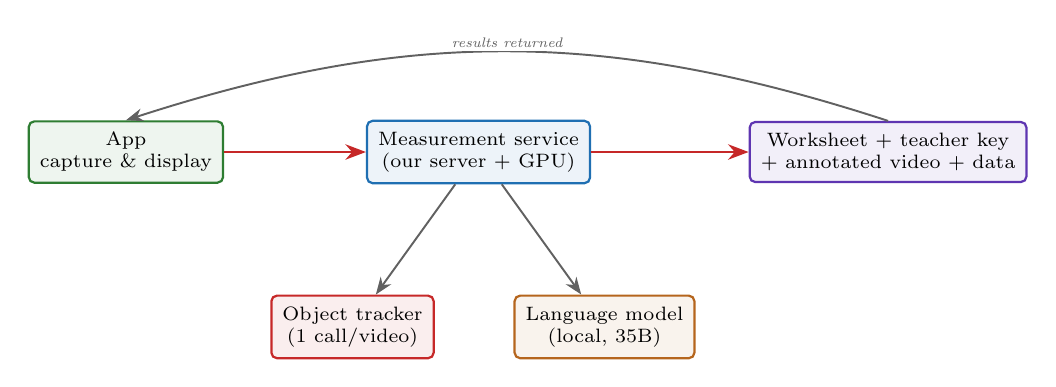
\begin{tikzpicture}[node distance=6mm and 16mm]
  \node[box=cApp] (app) {App\\capture \& display};
  \node[box=cMeas, right=18mm of app] (srv) {Measurement service\\(our server + GPU)};
  \node[box=cInfra, right=20mm of srv] (out) {Worksheet + teacher key\\+ annotated video + data};
  \node[box=cAccent, below=14mm of srv, xshift=-16mm] (trk) {Object tracker\\(1 call/video)};
  \node[box=cPed, below=14mm of srv, xshift=16mm] (llm) {Language model\\(local, 35B)};
  \draw[hot] (app)--(srv);
  \draw[hot] (srv)--(out);
  \draw[flow] (srv)--(trk);
  \draw[flow] (srv)--(llm);
  \draw[flow] (out.north) to[bend right=18] node[lbl,midway,above]{results returned} (app.north);
\end{tikzpicture}
\vspace{0.6em}
\begin{itemize}\setlength\itemsep{2pt}\footnotesize
  \item Everything runs on \emph{our own} lab infrastructure (GPU, tracker, the language model, the pipeline) --- no external paid API, no dependency on the original authors' servers.
  \item The language model is run \emph{locally} (privacy + cost + reproducibility); it is a 35-billion-parameter model served on a single workstation.
\end{itemize}
{\scriptsize (Networking note for the curious: public endpoint is tunnelled into the lab over a firewalled link; the tracker and the model sit on separate machines on the lab network.)}
\end{frame}

\begin{frame}{Under the hood --- the request lifecycle}
\centering
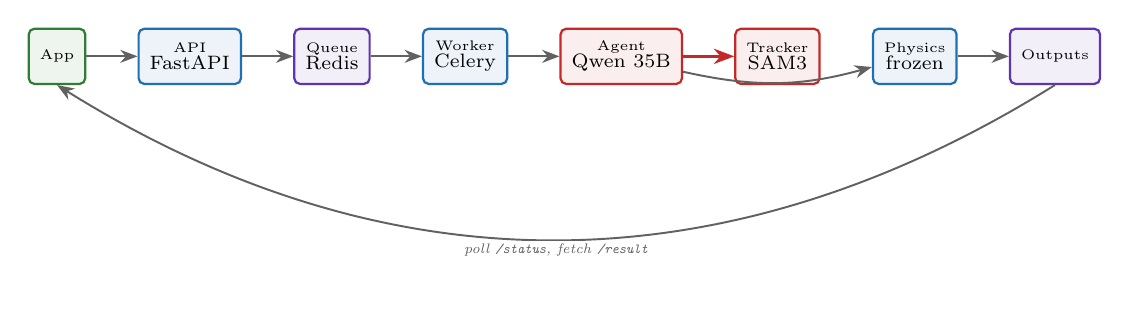
\begin{tikzpicture}[node distance=3mm and 6.5mm]
  \node[box=cApp, font=\tiny] (app) {App};
  \node[box=cMeas, font=\tiny, right=of app] (api) {API\\\scriptsize FastAPI};
  \node[box=cInfra, font=\tiny, right=of api] (q) {Queue\\\scriptsize Redis};
  \node[box=cMeas, font=\tiny, right=of q] (wk) {Worker\\\scriptsize Celery};
  \node[box=cAccent, font=\tiny, right=of wk] (ag) {Agent\\\scriptsize Qwen 35B};
  \node[box=cAccent, font=\tiny, right=of ag] (tr) {Tracker\\\scriptsize SAM3};
  \node[box=cMeas, font=\tiny, right=of tr] (fp) {Physics\\\scriptsize frozen};
  \node[box=cInfra, font=\tiny, right=of fp] (o) {Outputs};
  \draw[flow](app)--(api);\draw[flow](api)--(q);\draw[flow](q)--(wk);\draw[flow](wk)--(ag);
  \draw[hot](ag)--(tr);\draw[flow](ag) to[bend right=14](fp);\draw[flow](fp)--(o);
  \draw[flow](o.south) to[bend left=32] node[lbl,midway,below]{poll \texttt{/status}, fetch \texttt{/result}} (app.south);
\end{tikzpicture}
\vspace{0.4em}
\flushleft \footnotesize One job, end to end (real endpoints):
\begin{enumerate}\setlength\itemsep{1.5pt}\footnotesize
  \item App \texttt{POST /analyze} (video + sidecar) $\to$ API validates, creates an \emph{isolated workspace}, seeds the frozen physics module into it, enqueues a Celery job, returns \texttt{job\_id}
  \item App \texttt{GET /status/\{id\}} polls a live progress feed built from the agent's event stream
  \item Worker (Celery, \alert{one job at a time}) launches the \texttt{pi} agent inside that workspace
  \item Agent perception (Steps 1--5) writes \texttt{pipeline\_inputs.json}; then \texttt{python -m analysis.run} (Step 6) writes \texttt{stats.json} + \texttt{kinematics.csv}
  \item Parallel subagents render figures, annotated video, and learning material $\to$ LaTeX $\to$ student / teacher PDFs
  \item Result paths land in Redis; App \texttt{GET /result/\{id\}} fetches the PDFs / video / CSV via \texttt{/files}
\end{enumerate}
\end{frame}

\begin{frame}{Deployment \& infrastructure --- the full stack}
\small
\begin{columns}[T]
\column{0.48\textwidth}
{\footnotesize \textbf{Docker Compose services} (one host):}\\[3pt]
{\scriptsize
\renewcommand{\arraystretch}{1.15}
\begin{tabular}{@{}lll@{}}
\toprule
service & tech & role\\
\midrule
\texttt{caddy} & Caddy 2 & TLS reverse proxy (:80/:443)\\
\texttt{api} & FastAPI & REST + job intake (:8088)\\
\texttt{redis} & Redis 7 & broker + state/results (AOF)\\
\texttt{worker} & Celery & runs the agent, 1 job/time\\
\texttt{beat} & Celery & hourly workspace cleanup\\
\bottomrule
\end{tabular}}\par\vspace{6pt}
{\scriptsize \textbf{State \& storage:} each job gets a self-contained \emph{workspace} on disk (frozen code seeded in); job status + result JSON live in Redis (persisted); stale workspaces expire on a timer (\texttt{beat}).}
\column{0.52\textwidth}
\centering
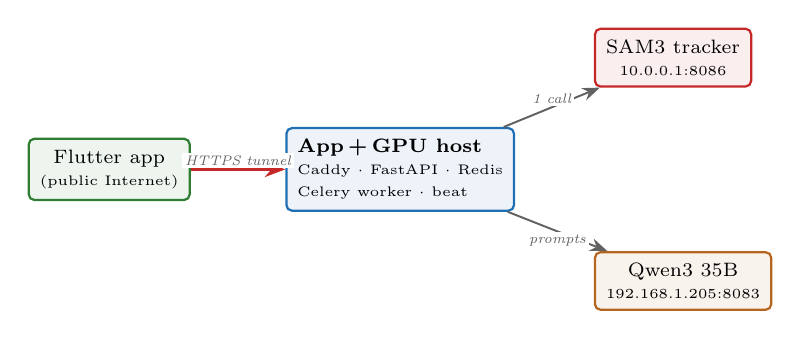
\begin{tikzpicture}[font=\scriptsize, node distance=4mm and 10mm]
  \node[box=cApp] (cl) {Flutter app\\\tiny (public Internet)};
  \node[box=cMeas, right=12mm of cl, align=left] (host) {\textbf{App\,+\,GPU host}\\\tiny Caddy $\cdot$ FastAPI $\cdot$ Redis\\\tiny Celery worker $\cdot$ beat};
  \node[box=cAccent, above right=5mm and 10mm of host] (tr) {SAM3 tracker\\\tiny 10.0.0.1:8086};
  \node[box=cPed, below right=5mm and 10mm of host] (llm) {Qwen3 35B\\\tiny 192.168.1.205:8083};
  \draw[hot] (cl) -- node[lbl,midway,above]{HTTPS tunnel} (host);
  \draw[flow] (host) -- node[lbl,midway,above]{1 call} (tr);
  \draw[flow] (host) -- node[lbl,midway,below]{prompts} (llm);
\end{tikzpicture}\\[4pt]
{\scriptsize Three machines: the app/GPU host runs the whole stack; the tracker and the 35B model sit on \emph{separate} lab GPUs. No external paid API.}
\end{columns}
\end{frame}

\begin{frame}{The agentic measurement pipeline (inside one job)}
\centering
\resizebox{0.74\linewidth}{!}{%
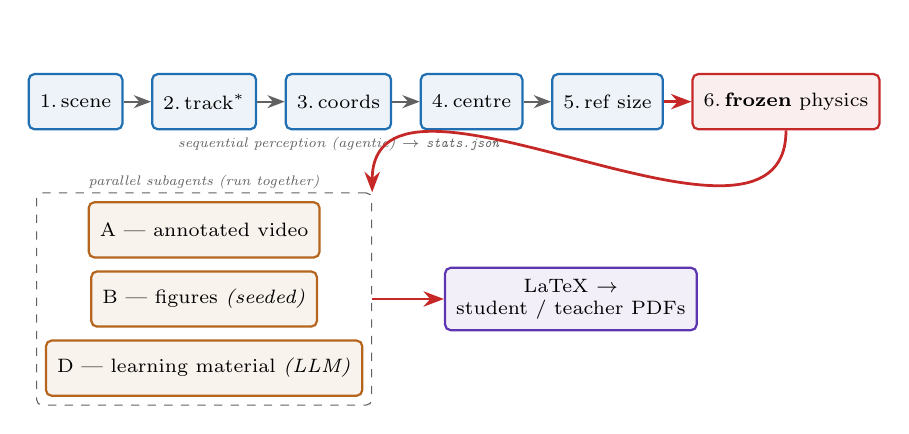
\begin{tikzpicture}[font=\tiny, node distance=3mm and 3.5mm]
  % tier 1 --- sequential perception then the frozen physics
  \node[box=cMeas] (s1) {1.\,scene};
  \node[box=cMeas, right=of s1] (s2) {2.\,track$^\ast$};
  \node[box=cMeas, right=of s2] (s3) {3.\,coords};
  \node[box=cMeas, right=of s3] (s4) {4.\,centre};
  \node[box=cMeas, right=of s4] (s5) {5.\,ref size};
  \node[box=cAccent, right=of s5] (s6) {6.\,\textbf{frozen} physics};
  \draw[flow](s1)--(s2);\draw[flow](s2)--(s3);\draw[flow](s3)--(s4);\draw[flow](s4)--(s5);\draw[hot](s5)--(s6);
  \node[lbl, below=0.5mm of s3] {sequential perception (agentic) $\rightarrow$ \texttt{stats.json}};
  % tier 2 --- the three subagents run in parallel (no arrows between them)
  \node[box=cPed, below=9mm of s2, minimum width=24mm] (A) {A --- annotated video};
  \node[box=cPed, below=1.5mm of A, minimum width=24mm] (B) {B --- figures \emph{(seeded)}};
  \node[box=cPed, below=1.5mm of B, minimum width=24mm] (C) {D --- learning material \emph{(LLM)}};
  \node[draw=cGrey, dashed, rounded corners=2pt, fit=(A)(B)(C), inner sep=3pt] (sa) {};
  \node[lbl, anchor=south] at (sa.north) {parallel subagents (run together)};
  % tier 3 --- compile
  \node[box=cInfra, right=16mm of B, minimum width=26mm] (tex) {LaTeX $\rightarrow$\\student / teacher PDFs};
  \draw[hot] (s6) to[out=-90,in=90] (sa.north east);
  \draw[hot] (sa.east) -- (tex.west);
\end{tikzpicture}}
\vspace{-0.4em}
\begin{columns}[T]
\column{0.5\textwidth}
{\footnotesize \textbf{Sequential perception (agentic)}}
\begin{itemize}\setlength\itemsep{1pt}\footnotesize
  \item Steps 1--5: the agent \emph{writes and runs its own Python}; $^\ast$tracker called \alert{once} and cached
  \item Step 6 is the \alert{frozen} module --- all kinematics, one locked schema
\end{itemize}
\column{0.5\textwidth}
{\footnotesize \textbf{Parallel rendering (then verify)}}
\begin{itemize}\setlength\itemsep{1pt}\footnotesize
  \item A (video) \& B (figures): \emph{seeded} code the agent runs, then \emph{visually QA-checks}
  \item D (learning material): the genuine LLM author, grounded by a deterministic seed; a verification loop gates LaTeX
\end{itemize}
\end{columns}
\vspace{1pt}
{\scriptsize\color{cAccent}\textbf{Planned:} extend the gate from figures/numbers to the \emph{material prose} (correct physics) --- until then, prose rests on the teacher panel.}
\end{frame}

% --- blank black slides (blackout buffer before the summary) ---
{\setbeamercolor{background canvas}{bg=black}\begin{frame}[plain]{}\end{frame}}
{\setbeamercolor{background canvas}{bg=black}\begin{frame}[plain]{}\end{frame}}
{\setbeamercolor{background canvas}{bg=black}\begin{frame}[plain]{}\end{frame}}

\begin{frame}[standout]{Summary}
\begin{itemize}\setlength\itemsep{6pt}
  \item One video $\to$ reproducible physics $\to$ multimodal, phenomenon-grounded learning material.
  \item Measurement already agrees with the gyroscope to \alert{0.3\%}; material relevance \alert{0.840} BERTScore vs.\ an authentic textbook.
  \item Evaluation deliberately mirrors the prior method (BERTScore relevance + \alert{10-teacher} panel, $\kappa$ / ANOVA / Pearson) for a fair comparison.
  \item Pedagogy preserved end-to-end: phenomenon-grounded, modality-tagged learning material, and a learning-effect study ready to run.
\end{itemize}
\end{frame}

% =========================================================================
% ==================  BACKUP / APPENDIX  (deferred slides)  ================
% =========================================================================
\appendix

\begin{frame}[standout]{Backup --- how the system works}
\centering
The slides that follow cover the measurement pipeline, tracking, the validation
cases and the infrastructure --- kept in reserve for questions on \emph{how} the
numbers are produced.
\end{frame}

% =========================================================================
\begin{frame}{The contribution, and the headline numbers}
\begin{block}{Claim}
A single ordinary \alert{video} of a rotating object replaces a phone gyroscope, and from
that one capture we recover the full motion \emph{and} auto-generate multimodal,
phenomenon-grounded learning material --- aligned with a prior multimodal method for a comparable study.
\end{block}
\vspace{0.4em}
\centering
\bignum{0.3\,\%}{video vs.\ gyroscope\\(mean $\omega$, IMG\_3075)}\hfill
\bignum{93.8\,\%}{tracking coverage\\(bicycle clip)}\hfill
\bignum{5}{multimodal\\sections / scene}
\vspace{0.6em}
\begin{columns}[T]
\column{0.5\textwidth}
{\footnotesize \textbf{What is new vs.\ the prior method:}}
\begin{itemize}\setlength\itemsep{1pt}\footnotesize
  \item replaces the \emph{sensor} modality with \emph{video} --- no hardware, no calibration step
  \item one capture yields object + radius \emph{and} $\omega(t),a_c(t)$ --- two captures collapsed into one
\end{itemize}
\column{0.5\textwidth}
{\footnotesize \textbf{What is kept identical for fair comparison:}}
\begin{itemize}\setlength\itemsep{1pt}\footnotesize
  \item the centripetal-acceleration topic and the multimodal learning-material format
  \item the evaluation battery (BERTScore relevance + teacher panel)
\end{itemize}
\end{columns}
\end{frame}

\begin{frame}{Outline}
\setbeamertemplate{section in toc}[sections numbered]
\tableofcontents
\end{frame}

% =========================================================================
\section{Three methods, one pipeline}

\begin{frame}{The whole system is three methods chained}
\centering
\resizebox{\textwidth}{!}{%
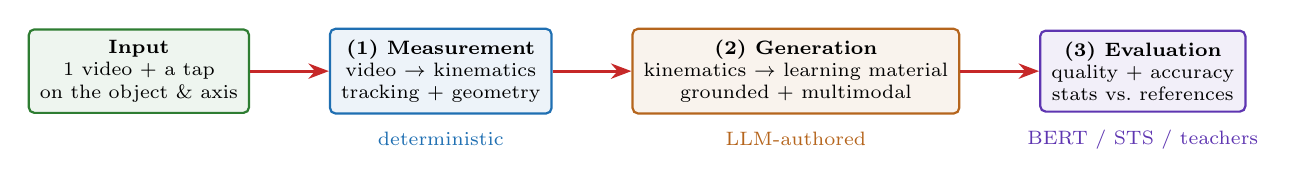
\begin{tikzpicture}[node distance=4mm and 10mm]
  \node[box=cApp, minimum width=24mm] (vid) {\textbf{Input}\\1 video + a tap\\on the object \& axis};
  \node[box=cMeas, right=of vid, minimum width=26mm] (m1) {\textbf{(1) Measurement}\\video $\to$ kinematics\\\scriptsize tracking + geometry};
  \node[box=cPed, right=of m1, minimum width=26mm] (m2) {\textbf{(2) Generation}\\kinematics $\to$ learning material\\\scriptsize grounded + multimodal};
  \node[box=cInfra, right=of m2, minimum width=26mm] (m3) {\textbf{(3) Evaluation}\\quality + accuracy\\\scriptsize stats vs.\ references};
  \draw[hot] (vid)--(m1); \draw[hot] (m1)--(m2); \draw[hot] (m2)--(m3);
  \node[below=1mm of m1, font=\scriptsize, text=cMeas] {deterministic};
  \node[below=1mm of m2, font=\scriptsize, text=cPed] {LLM-authored};
  \node[below=1mm of m3, font=\scriptsize, text=cInfra] {BERT / STS / teachers};
\end{tikzpicture}}
\vspace{0.8em}
\begin{itemize}\setlength\itemsep{4pt}
  \item \textcolor{cMeas}{\textbf{Measurement}} is \emph{reproducible code}, not an AI guess --- same video gives the same numbers byte-for-byte.
  \item \textcolor{cPed}{\textbf{Generation}} is the only place a language model writes content; it is grounded in the measured numbers.
  \item \textcolor{cInfra}{\textbf{Evaluation}} mirrors the prior method's methodology so the two systems can be compared directly.
\end{itemize}
\vspace{0.3em}
{\scriptsize Three questions guide the rest of the talk --- \emph{which method?}, \emph{what numbers?}, \emph{is it pedagogically sound?} --- one per box.}
\end{frame}

% =========================================================================
\section{Method 1 --- Measurement (video $\rightarrow$ physics)}

\begin{frame}{How the motion is measured (method, not code)}
\small
\begin{enumerate}\setlength\itemsep{4pt}
  \item \textbf{Track} the moving object across every frame (open-vocabulary detector + mask propagation) --- one call per video.
  \item \textbf{Fit the circular path} by RANSAC circle-fitting; reject points off the orbit ($>2.5\sigma$ or $>15$\,px $\to$ discarded, never guessed).
  \item \textbf{Calibrate} pixels to metres using a reference object of known size: $\;\text{px\_per\_m}=\dfrac{\text{diameter}_{\text{px}}}{\text{size}_{\text{m}}}$.
  \item \textbf{Differentiate the angle} to get angular velocity, then the rest follows from physics:
\end{enumerate}
\vspace{-0.2em}
\[
\theta=\operatorname{unwrap}\big(\operatorname{atan2}(\Delta y,\Delta x)\big),\qquad
\omega=\frac{d\theta}{dt},\qquad
v=\lvert\omega\rvert\,r,\qquad
\boxed{\,a_c=\omega^{2} r\,}.
\]
\vspace{-0.2em}
\begin{columns}[T]
\column{0.62\textwidth}
{\footnotesize \textbf{Signal-processing choices (the methodological details):}}
\begin{itemize}\setlength\itemsep{1pt}\footnotesize
  \item Savitzky--Golay smoothing of $\theta$ (window $\approx$ fps/6) before differentiating
  \item one $\omega$ series drives \emph{every} downstream number (no internal inconsistency)
  \item period $T=\dfrac{2\pi}{\operatorname{median}|\omega|}$, cross-checked by an FFT of $\theta(t)$
\end{itemize}
\column{0.38\textwidth}
\centering
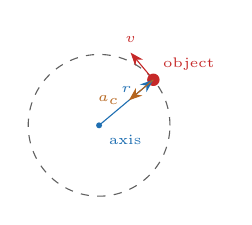
\begin{tikzpicture}[scale=0.9]
  \draw[cGrey,dashed] (0,0) circle (1.0);
  \fill[cMeas] (0,0) circle (1.2pt) node[below right,font=\tiny]{axis};
  \fill[cAccent] (40:1.0) circle (2.5pt) node[above right,font=\tiny]{object};
  \draw[-{Stealth},cMeas] (0,0)--(40:1.0) node[midway,above,font=\tiny]{$r$};
  \draw[-{Stealth},cAccent] (40:1.0)--($(40:1.0)+(130:0.5)$) node[above,font=\tiny]{$v$};
  \draw[-{Stealth},cPed] (40:1.0)--($(40:1.0)+(220:0.45)$) node[left,font=\tiny]{$a_c$};
\end{tikzpicture}
\end{columns}
\end{frame}

\begin{frame}{Measurement internals --- the exact recipe}
\scriptsize
The whole quantitative path is one frozen module (\texttt{python -m analysis.run}). Every constant below is fixed in code, so the run is deterministic.
\vspace{0.2em}
\begin{columns}[T]
\column{0.5\textwidth}
\textbf{\color{cMeas}Geometry \& calibration}
\begin{itemize}\setlength\itemsep{1.5pt}
  \item \textbf{Circle fit:} RANSAC on a 3-point \emph{circumcircle}, 1000 iters, inlier band $|d-r|<\SI{8}{px}$; accept if $\ge\max(20,\,15\%\,\text{of valid})$ inliers
  \item \textbf{Degeneracy guard:} reject a fit with $r_{\text{fit}}>2\times$ the farthest point from the mark (a huge circle is locally a line and ``fits'' an arc)
  \item \textbf{Centre rule:} keep the human tap \emph{unless} the fit is unambiguously better ---
  \[\underbrace{\tfrac{\sigma_r}{\bar r}\Big|_{\text{fit}}<0.10}_{\text{tight}}\;\wedge\;\underbrace{\tfrac{\sigma_r}{\bar r}\Big|_{\text{fit}}<0.6\,\tfrac{\sigma_r}{\bar r}\Big|_{\text{mark}}}_{\text{lower scatter}}\]
  \item \textbf{Outliers:} drop $|r-\tilde r|>\max(2.5\sigma_r,\SI{15}{px})$; never extrapolate
  \item \textbf{Scale:} $\text{px\_per\_m}=\text{diameter}_\text{px}/\text{size}_\text{m}$ (reference object)
\end{itemize}
\column{0.5\textwidth}
\textbf{\color{cMeas}Kinematics \& motion model}
\begin{itemize}\setlength\itemsep{1.5pt}
  \item \textbf{Angle:} $\theta=\operatorname{unwrap}\operatorname{atan2}(\Delta y,\Delta x)$, per contiguous track segment
  \item \textbf{Smoothing:} Savitzky--Golay (window $\approx$ fps$/6$, order 3) on $\theta$, then $\omega=d\theta/dt$, then a median filter ($\approx$ fps$/10$). \alert{One} $\omega$ feeds every number
  \item \textbf{Gap fill:} interior dropouts $\le\SI{0.2}{s}$ interpolated in \emph{polar} $(\theta,r)$ --- points land on the arc, not the chord
  \item \textbf{Period:} $T=2\pi/\operatorname{median}|\omega|$, cross-checked by an FFT of detrended $\theta(t)$
  \item \textbf{Motion model:} fit $\theta(t)$ to a line vs.\ a parabola; declare non-uniform iff residual variance drops $>70\%$ \emph{and} $|\alpha|\,\Delta t/\bar\omega>0.3$; then report $\alpha$ and $a_t=\alpha r$
\end{itemize}
\end{columns}
\end{frame}

\begin{frame}{Tracking $\rightarrow$ geometry, on a real clip (the fan)}
\centering
\begin{columns}[c]
\column{0.5\textwidth}
\centering
\includegraphics[height=0.62\textheight]{fan_annotated_image}\\
{\scriptsize Scene geometry: per-frame tracked centroids, the RANSAC-fitted orbit (green), recovered axis at centre.}
\column{0.5\textwidth}
\centering
\includegraphics[height=0.62\textheight]{fan_trajectory}\\
{\scriptsize Orbit in metric space. The inward spiral is the doll \emph{swinging out} as the fan accelerates; the dashed circle is the fitted steady radius.}
\end{columns}
\vspace{0.3em}
{\scriptsize Both panels are \emph{actual pipeline output} for job \texttt{a2627aa2} --- not mock-ups.}
\end{frame}

\begin{frame}{Why the numbers are trustworthy: reproducibility by design}
\begin{columns}[T]
\column{0.52\textwidth}
\textbf{If a language model authored the physics} (the tempting shortcut):
\begin{itemize}\setlength\itemsep{2pt}
  \item output schema drifts run-to-run --- \hl{$\sim$28} formats over \hl{30} runs
  \item invalid / non-finite values slip through (\hl{$>$half} of runs)
  \item the estimated rotation centre can swing \hl{8.9 $\to$ 1013\,px} \emph{on the same video}
\end{itemize}
\column{0.48\textwidth}
\textbf{Physics as audited, frozen code} (the design):
\begin{itemize}\setlength\itemsep{2pt}
  \item \hl{1} locked output schema
  \item \alert{same video $\Rightarrow$ identical numbers} every run
  \item the language model only does perception; it never touches the physics
\end{itemize}
\end{columns}
\vspace{0.6em}
\begin{exampleblock}{\small Methodological stance}
{\small The language model is used \emph{only} where it is genuinely better than code
(recognising an arbitrary object from a text description, and writing natural-language learning material).
Everything quantitative is deterministic and verifiable --- this is what makes the measurement
defensible as a scientific instrument.}
\end{exampleblock}
\end{frame}

\begin{frame}{Measurement validation --- the accuracy pilot}
\small
\textbf{Design.} Same physical spin filmed \emph{and} recorded with the phone gyroscope; a constant-RPM
source (turntable / record player at \SI{33.3}{rpm}) gives an \alert{absolute} ground truth for both legs.
\begin{itemize}\setlength\itemsep{2pt}
  \item \textbf{Summary-stats comparison first} (mean $\omega$, period, revolutions) --- answers ``good enough?'' with no clock sync.
  \item \textbf{Time-series later}, aligned by \alert{cross-correlation} (robust to phone-clock drift), not wall-clock timestamps.
  \item Statistic of record: \textbf{Pearson $r$} and percentage error between video and sensor.
\end{itemize}
\vspace{0.3em}
\centering
\bignum{0.3\,\%}{video vs.\ gyro\\mean $\omega$ (IMG\_3075)}\hfill
\bignum{93.8\,\%}{coverage\\(bicycle clip)}\hfill
\bignum{1.18\,s}{period\\(0.85\,Hz)}\hfill
\bignum{1.9--2.1}{$a_c$ (m/s$^2$)\\bicycle}
\vspace{0.4em}
\flushleft
{\scriptsize Ground truth lives outside the system and is never shown to the AI --- so the agreement is a genuine external check, not a fit.}
\end{frame}

\begin{frame}{The tracking method --- a wording finding (with numbers)}
\small
The detector is \emph{open-vocabulary}: it matches the \textbf{words} you give it to regions of the image.
So the wording of the object description is, empirically, the single biggest lever on reliability.
\vspace{0.4em}
\centering
{\footnotesize \textbf{Same fan clip, same frames --- coverage by prompt wording:}}\\[2pt]
\begin{tabular}{@{}lcc@{}}
\toprule
prompt & detector A (LocateAnything) & production detector (SAM3)\\
\midrule
\texttt{"cream colored doll"} & 6\,\% & ---\\
\texttt{"doll"} & 70\,\% & \hl{0\,\%}\\
\texttt{"toy"} & \hl{100\,\%} & \hl{0\,\%}\\
\texttt{"yellow toy"} / \texttt{"hanging toy"} & --- & \hl{100\,\%}\\
\bottomrule
\end{tabular}
\vspace{0.5em}
\flushleft
\begin{itemize}\setlength\itemsep{2pt}\footnotesize
  \item A \alert{16$\times$} swing (6\% $\to$ 100\%) from \emph{wording alone} --- not resolution, not the camera.
  \item The best wording is \emph{detector-specific}: one model likes \texttt{"toy"}, the production model needs \texttt{"yellow toy"}.
  \item \textbf{What we do now:} probe a few candidate words \emph{manually} on $\sim$12 sampled frames before committing --- a small, cheap calibration of language to model. \emph{Automating this micro-sweep in the pipeline is on the roadmap.}
\end{itemize}
\end{frame}

\begin{frame}{Robustness: self-correcting geometry, and non-uniform motion}
\scriptsize
Two failures that \emph{look} like noisy data are really \emph{model} mismatches --- both now handled, turning the hardest clip into the richest one.
\vspace{0.1em}
\begin{columns}[T]
\column{0.52\textwidth}
\textbf{(a) The rotation centre self-corrects}
\begin{itemize}\setlength\itemsep{1.5pt}
  \item a hand-tapped axis can sit \emph{off} the orbit centre --- here \hl{158\,px} off
  \item measuring $r,\theta,\omega$ about the wrong centre \emph{fakes} an unstable radius (scatter \hl{39\,\%})
  \item the fit replaces the mark only when clearly better $\Rightarrow$ scatter \hl{39\,\%\,$\to$\,10\,\%}
\end{itemize}
\vspace{2pt}
\textbf{(b) Non-uniform spin is measured, not dismissed}
\begin{itemize}\setlength\itemsep{1.5pt}
  \item the fan \emph{spins up}: constant $\alpha=$\,\hl{1.18}\,rad/s$^2$, fit $R^2=$\,\hl{0.9999}
  \item the same test catches turntables \emph{coasting down} ($\alpha\approx$\,\hl{$-4$})
\end{itemize}
\vspace{-0.1em}
\[ a_t=\alpha r,\quad a_c=\omega^2 r,\quad a=\sqrt{a_t^2+a_c^2}. \]
\column{0.48\textwidth}
\centering
\includegraphics[width=\linewidth]{fan_omega}\\
{\scriptsize Measured $\omega(t)$ for the fan: a clean ramp \hl{3.2$\to$10.2}\,rad/s (dashed = mean, shown only for reference). A single ``stable $\omega$'' would be wrong here --- the parabola-vs-line test detects this and reports $\alpha$ instead.}
\end{columns}
\vspace{0.1em}
{\scriptsize Beyond the steady-rotation assumption of the prior method: both acceleration components are available, so the learning material can teach angular acceleration from the phenomenon.}
\end{frame}

% =========================================================================
\section{Validation across cases}

\begin{frame}{Three real cases span the three motion regimes}
\scriptsize One pipeline, \emph{no per-case tuning}; the measured $\omega(t)$ is each scene's signature.
\vspace{0.3em}
\centering
\renewcommand{\arraystretch}{1.25}
\begin{tabular}{@{}lcccccc@{}}
\toprule
case & regime & coverage & $\omega$ & period & $r$ & $a_c$\\
\midrule
\textbf{\color{cApp}Bicycle wheel} (driven) & \hl{uniform} & 93.8\,\% & $\approx$5.1\,rad/s & 1.18\,s & 0.075\,m & 1.9--2.1\\
\textbf{\color{cAccent}Turntable} (hand-spun) & \hl{decelerating} & 100\,\% & 8.1\,$\to$\,2.2\,rad/s & 1.37\,s & 0.148\,m & 3.99\\
\textbf{\color{cPed}Ceiling fan} (powered) & \hl{accelerating} & 100\,\% & 3.2\,$\to$\,10.2\,rad/s & 0.91\,s & 1.84\,m$^\ast$ & 88.5\\
\bottomrule
\end{tabular}
\vspace{0.5em}
\flushleft
{\scriptsize Constant-$\omega$, constant-$\alpha$ decay, and constant-$\alpha$ growth --- all three recovered by the same parabola-vs-line test. \;$^\ast$fan radius uses a provisional reference size; $\omega,\alpha,T$ are scale-free.}
\end{frame}

\begin{frame}{Case 1 --- bicycle wheel: \emph{uniform} circular motion}
\centering
\begin{columns}[c]
\column{0.34\textwidth}\centering
\includegraphics[width=\linewidth]{bike_annotated_image}\\{\scriptsize scene + fitted orbit}
\column{0.40\textwidth}\centering
\includegraphics[width=\linewidth]{bike_omega}\\{\scriptsize $\omega(t)$ flat --- steady driven wheel}
\column{0.26\textwidth}
\scriptsize
\textbf{Driven wheel} --- constant speed.
\begin{itemize}\setlength\itemsep{2pt}
  \item $\omega\approx$\,\hl{5.1}\,rad/s, $T=$\,\hl{1.18}\,s
  \item $a_c\approx$\,\hl{1.9--2.1}\,m/s$^2$
  \item coverage \hl{93.8\,\%}
  \item line fit of $\theta(t)$ suffices ($\alpha\approx0$)
\end{itemize}
\end{columns}
\vspace{0.2em}
{\scriptsize \textbf{What the agent did:} read the clip, tracked the marker as \texttt{``red object''} across every frame, fit the orbit by RANSAC; finding $\theta(t)$ already straight, it classified the motion \emph{uniform} --- the classic $a_c=\omega^2 r$ is the whole story.}
\end{frame}

\begin{frame}{Case 2 --- turntable: \emph{decelerating} (a hand-spin coasting down)}
\centering
\begin{columns}[c]
\column{0.34\textwidth}\centering
\includegraphics[width=\linewidth]{tt_annotated_image}\\{\scriptsize scene + fitted orbit}
\column{0.40\textwidth}\centering
\includegraphics[width=\linewidth]{tt_omega}\\{\scriptsize $\omega(t)$: a push, then free coast-down}
\column{0.26\textwidth}
\scriptsize
\textbf{Hand-spun disc} --- friction brakes it.
\begin{itemize}\setlength\itemsep{2pt}
  \item $\omega$ \hl{8.1\,$\to$\,2.2}\,rad/s
  \item $\alpha\approx$\,\hl{$-3.3$}\,rad/s$^2$
  \item $T=$\,\hl{1.37}\,s, coverage \hl{100\,\%}
  \item tangential $a_t=\alpha r$ now reported too
\end{itemize}
\end{columns}
\vspace{0.2em}
{\scriptsize \textbf{What the agent did:} tracked the \texttt{``red phone''}, fit the disc centre, then saw $\theta(t)$ bend over time --- it fit a parabola, reported $\alpha<0$, and labelled the run a \emph{coast-down} that a single mean-$\omega$ would have smeared.}
\end{frame}

\begin{frame}{Case 3 --- ceiling fan: \emph{accelerating} (powered spin-up)}
\centering
\begin{columns}[c]
\column{0.34\textwidth}\centering
\includegraphics[width=\linewidth]{fan_annotated_image}\\{\scriptsize scene + fitted orbit; centre auto-corrected}
\column{0.40\textwidth}\centering
\includegraphics[width=\linewidth]{fan_omega}\\{\scriptsize $\omega(t)$: a clean ramp up}
\column{0.26\textwidth}
\scriptsize
\textbf{Powered fan} --- spins up from rest.
\begin{itemize}\setlength\itemsep{2pt}
  \item $\omega$ \hl{3.2\,$\to$\,10.2}\,rad/s
  \item $\alpha=$\,\hl{1.18}\,rad/s$^2$ ($R^2$\,\hl{0.9999})
  \item \hl{100\,\%} tracking; \hl{158\,px} off-axis mark auto-corrected
  \item the hardest clip --- all robustness features at once
\end{itemize}
\end{columns}
\vspace{0.2em}
{\scriptsize \textbf{What the agent did:} tracked the \texttt{``yellow toy''}, noticed the tapped axis sat \hl{158\,px} off the fitted circle and \emph{auto-corrected} it, then the parabola fit revealed a clean \emph{spin-up} ($\alpha=1.18$) --- all three robustness features firing on one clip.}
\end{frame}

\begin{frame}{Reading the kinematic readout (the fan, as an example)}
\centering
\begin{columns}[c]
\column{0.5\textwidth}\centering
\includegraphics[width=0.82\linewidth,height=0.33\textheight,keepaspectratio]{fan_theta}\\[1pt]
{\scriptsize $\theta(t)$ --- total angle turned; its \emph{curvature} is the acceleration}\\[5pt]
\includegraphics[width=0.82\linewidth,height=0.33\textheight,keepaspectratio]{fan_ac}\\[1pt]
{\scriptsize $a_c(t)=\omega^2 r$ --- rises as the fan speeds up}
\column{0.5\textwidth}\centering
\includegraphics[width=0.82\linewidth,height=0.33\textheight,keepaspectratio]{fan_omega}\\[1pt]
{\scriptsize $\omega(t)=d\theta/dt$ --- the ramp; its \emph{slope} is $\alpha$}\\[5pt]
\includegraphics[width=0.82\linewidth,height=0.33\textheight,keepaspectratio]{fan_trajectory}\\[1pt]
{\scriptsize orbit in metres --- points sit on the fitted circle}
\end{columns}
\vspace{0.1em}
{\scriptsize Every run emits this readout. $\theta\!\to\!\omega\!\to\!a_c$ is one consistent chain; the four views cross-check each other.}
\end{frame}


\end{document}
